\documentclass[a4paper,12pt,twoside]{extarticle}
\usepackage{fontspec}
\usepackage{calc}
\newlength{\lengthwidth}
\setlength{\lengthwidth}{\textwidth - 11em}
\usepackage[framemethod=tikz]{mdframed}
\usetikzlibrary{calc}
\usepackage{graphicx}
\usepackage{longtable}
\usepackage[strict]{changepage}
\usepackage{lipsum}
\usepackage{multicol}
\usepackage{multirow}
\usepackage[cm]{fullpage}
\usepackage[english]{babel}
\usepackage{amsmath,amsfonts,amsthm}
\usepackage[document]{ragged2e}
\usepackage{booktabs}
\usepackage{fix-cm}
\usepackage[none]{hyphenat}
\usepackage{fancyhdr}
\pagestyle{fancy}
\usepackage{lastpage}
\usepackage[export]{adjustbox}
\usepackage{caption}
\captionsetup[figure]{slc=off}
\usepackage[hidelinks]{hyperref}
\usepackage{titling}
\usepackage{mdframed}
\usepackage[]{quoting}
\newcommand{\thedate}{\today}
\setlength\LTleft{13.5em}
\definecolor{mycolor}{RGB}{238, 233, 233}
\definecolor{RoyalBlue}{RGB}{65, 105, 255}



\fancyfoot{}
\fancyfoot[LE]{\scriptsize{\textit{Reaudito}}}
\fancyfoot[LO]{\scriptsize{\textit{Reaudito}}}
\fancyfoot[RE,RO]{\footnotesize Page \thepage\ of \pageref*{LastPage}}
\renewcommand{\headheight}{14.5pt}
\renewcommand{\headrulewidth}{0.0pt}
\renewcommand{\footrulewidth}{0.4pt}
\fancypagestyle{firststyle}
{
   \fancyhf{}
   \fancyfoot[LO]{\scriptsize{\textbf{Cite this Article as: }\textit{Amiya Behera(2020) Avrit: The blockchain-based decentralized education system
   }}} }
\hypersetup{pdftitle={Avrit: The blockchain-based decentralized education system}, pdfauthor={Amiya Behera},pdfsubject={Education System}, pdfkeywords = {education, learning strategies, evidence of learning}, pdfcreator = {I am Brainstorming},pdfproducer={I am Brainstorming}}






\mdfdefinestyle{abstractstyle}{linecolor=RoyalBlue,
				  backgroundcolor=mycolor,
				  linewidth = 2pt,
				  rightline = false,
				  leftline = false,
				  frametitle=Abstract,
				  frametitlerule= true}
\mdfdefinestyle{captionstyle}{linecolor=RoyalBlue,
				  backgroundcolor=mycolor,
				  linewidth = 1pt,
				  rightline = false,
				  leftline = false}

\begin{document}
\sloppy
\begin{adjustwidth}{11em}{}


\thispagestyle{firststyle}




\LARGE{\textbf{\textcolor{RoyalBlue}{Avrit: The blockchain-based decentralized education system}}}\\[5mm]



\footnotesize{Amiya Behera\textsuperscript{*},\textsuperscript{
\includegraphics[width=9pt]{mail.png}}}
\\
\scriptsize{\textsuperscript{*} Blockchain Developer, Reaudito (https://avrit.reaudito.com)\\[5mm]}
\centering\textbf{\thedate}


\footnotesize{
\begin{mdframed}[style=abstractstyle]
\textbf{Avrit is a decentralized education system to be built on the top blockchain that evaluates evidence of learning and quality of curriculum; provides a collaboration platform for teachers, students, researchers, and rentable educational resource providers.  It relies on game-theoretic incentive systems where participants earn for the quality contribution they make to the platform.}
\end{mdframed}
}
\raggedright
  \footnotesize{\textbf{\textcolor{RoyalBlue}{Article Type:}}}
  \footnotesize{Research}  \\
	\footnotesize{\textbf{\textcolor{RoyalBlue}{Subject:}}} \footnotesize{Decentralized Education System} \\[10pt]
	 

 \footnotesize{\textbf{Keywords:}} \footnotesize{education, learning strategies, evidence of learning}  \\

 \section*{Introduction}
 \begin{quoting}
 I tell my students, 'When you get these jobs that you have been so brilliantly trained for, just remember that your real job is that if you are free, you need to free somebody else. If you have some power, then your job is to empower somebody else. This is not just a grab-bag candy game.
 -- Toni Morrison
\end{quoting}



 Education is a process of acquiring knowledge; developing reasoning skills for making good judgments; and acquisition of necessary skills, values, beliefs, and habits.
The current education system faces serious problems of quality, resource crunch and educational malpractices which includes obsolete teaching, substandard centralized curriculum and learning material, high-stake standardized exams that limit exploration and original thinking, mass cheating in exams and projects, appalling teacher and student ratio, poor classroom infrastructure, and non-availability of classrooms and specialized courses nearby students residence.

 
 
 \section*{Competitive Collaboration}
 It's a decentralized network where you compete to collaborate.

 Edge weight represents difficulty to get connected. Difficulty depends on factors such as distance, location, quality, price.
 We need to choose a subgraph containing all the required nodes (e.g. nodes containing a,b,c,d ) that has a minimum weight or optimal weight.
 

 
 \begin{figure}[h]\begin{adjustwidth}{11em}{}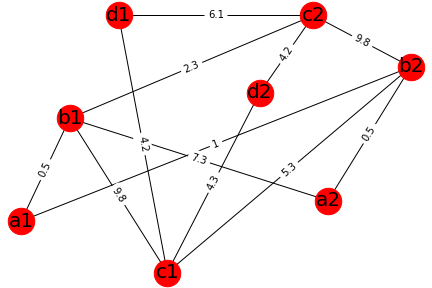
\includegraphics[width=\lengthwidth]{graph.png}\begin{mdframed}[style=captionstyle]\caption*{  \scriptsize \textit{\textbf{Figure: }Pick the minimum weight subgraph}}\end{mdframed}\end{adjustwidth}\end{figure}
    a,b,c,d can represent different services, whereas a1, a2 represents the same services from a different service provider.


    For example,\\
    ‘a’ can represent a student, ‘b’ can represent a teacher, ‘c’ can represent content provider such as a biology textbook and ‘d’ can represent a classroom or building.
    Similarly ‘b1’ represents teacher1, ‘b2’ represents teacher2, etc.
    
\subsubsection*{Usefulness of the model}
1) Predictive: One can make a prediction using the model, to select the best subgraph or services for an individual. Entrepreneurs can use the data to set up new nodes, based on the requirements of people. Policymakers can use the data to evaluate the quality and provide suggestions for the optimal functioning of the network.

2) Equal chance to everyone: Its fairer and everyone can get an equal chance to reach their goals. It will bring competition for quality. Equal chance means many selected subgraphs for many individuals will have similar weight, the possibility of getting similar weight increases when we increase the nodes.

3) Continuous Improvement: If any single subgraph, even a node of subgraph gets upgraded and refined, it builds pressure on other subgraph and nodes to upgrade through competition.

4) No burnouts: Nodes shall not suffer from burnout problems as there is a division of work between people and a division of labor.

5) Non-hierarchical and autonomous: As different nodes are independent of each other and are free to connect to other nodes, there is no hierarchy or concentration of power or monopoly.

6) Updated and Validated information: Nodes can be created after KYC, and they can make connections using their account after predicting the best weights or edges for them. The information will be validated using Schelling Game incentive models.

7) No information asymmetry: All data and evidence of learning remain open access, which makes an ideal price discovery. 

8) Collaboration, not competition: In a competition, some get the advantage while others are not given the chance to succeed.  But, competing against (someone) is not the same as competing for (something). It's a collaborative game, where optimal results are obtained through collaboration. Here, people compete for collaboration and quality. 

9) Updated and Validated information: Nodes are protected by game-theoretic incentive system, those who behave frivolously are punished.
\section*{Smart Contract}

Avrit will use its own native token to incentivize teachers, students, academicians, and content creators. Teachers can demand any number of tokens from students. But tokens will remain in escrow, until evidence of learning of students is validated and approved every month. Validation is done through Schelling Game incentive models similar to Kleros courts. \\ 
Kid's accounts can be delegated by parents, and students also receive tokens after evaluation for submitting their evidence of learning. 

\begin{figure}[h]\begin{adjustwidth}{11em}{}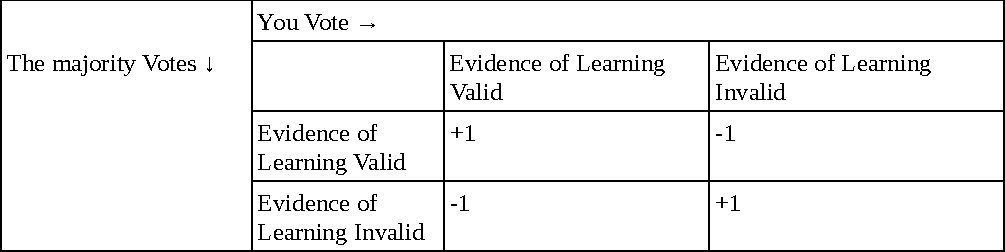
\includegraphics[width=30em]{shelling_game_avrit.pdf}\begin{mdframed}[style=captionstyle]\caption*{  \scriptsize \textit{\textbf{Figure: Shelling game }}}\end{mdframed}\end{adjustwidth}\end{figure}


There will be a total of two court types: \\
 \\  \\ 
\textbf{Profile auditing court:}  \\
This court will check the authenticity of profiles which can include specialization of teachers. If a profile is found malicious, it will be kept on hold, and can't receive any incentives until the dispute is solved. 
\\  \textbf{Reviewing the review court:} \\
Reviewers can apply to gain incentives if they have done a quality review and the court will judge the quality and grant incentive to the reviewer. Anyone is free to review the quality of the curriculum and evidence of learning. But review quality is accessed by “reviewing the review” courts, and only best reviews are used to decide the quality. 



\section*{Criteria for Reviewing:}

1) Pairing graphics with words:\\
Students learning increases when they receive information that includes both visual and texts. Graphics can include illustrations, diagrams, and flow charts, etc.

2) Linking abstract concepts with concrete representation:\\
Concrete examples help a student to understand new ideas, and apply the concepts in new situations.

3)Posing probing questions: \\
Quality questions that create curiosity to probe into the topic.
Asking questions like how, why, what if, why not, how do you know, what are the evidence, to analyze, process and decide things along with finding alternatives solutions. 

4) Repeatedly alternating problems with their solution provided and problems that students must solve. \\
Use interleaving and component practice for better transfer of learning with appropriate cognitive load.

5) Distributing practice \\
Asking students to revise and retrieve multiple times through spacing. It helps improve student retention

6) Assessing to boost retention \\
Testing students with questions about how they have learned.
\\
\textbf{More details and features with elaboration can be found in the blog:} \\
https://tinyurl.com/uxk3jgm

\section*{Governance by teachers and academician}

Teacher and academician committees are selected based on approval voting (seq-phragmen algorithm). Their job is to review the evidence of learning, curriculum, and quality of study centers. They also approve certification at the end of the course. Students need to upload their evidence of learning every week till they complete the course. 

\section*{Interface components of App}


\textbf{Curriculum:}

It includes:

1) Learning objectives i.e. knowledge and skills students are expected to learn.

2) Prior knowledge required to pursue the curriculum

3) References which can include chapters of books, videos, MOOCs, magazine articles, or research articles

4) Test and assessments and other methods to evaluate student learning

\textbf{Evidence of Learning:}

Students will upload evidence of learning that must be unplagiarized.

Learning evidence must be the work of the student in question. It can be any format like videos, audios, text, pdf, images. Multiple formats and evidence types are required. Evidence must be made that favors the discovery of authentication like using own voice in video or audio

\textbf{Peer Review:}

The evidence of learning and curriculum will undergo peer review to check whether it meets the learning standard as per learning strategies criteria. Money in escrow is transferred to teachers and students gain incentive only after evidence of learning is found to be of a high standard. 



\section*{\textcolor{RoyalBlue}{References}}
\begin{scriptsize}
\begin{enumerate} 
\item Kleros, \href{https://kleros.io/en/}{https://kleros.io/en/}
\item \href{https://blog.ethereum.org/2015/01/28/p-epsilon-attack/}{The P + epsilon Attack by Vitalik Buterin on January 28, 2015} 
\item Features of good books \href{https://tinyurl.com/uxk3jgm}{https://tinyurl.com/uxk3jgm}
\item Learning About Learning, National Council of Teacher Quality
\item Learning Scientists \href{https://www.learningscientists.org/}{https://www.learningscientists.org/}
\item Jacob, Brian A. and Steven D. Levitt (Winter 2004). “To Catch a Cheat”. Education Next
\item Tierney, William G., and Nidhi Sadana Sabharwal. “Academic corruption: Culture and trust in Indian higher education.“ International Journal of Educational Development 55 (2017): 30-40.
\item Ehrenberg, Ronald G. et al. “Class Size and Student Achievement.” Psychological science in the public interest : a journal of the American Psychological Society 2 1 (2001): 1-30 .
\item Making (Low-Stakes) Practice Tests More Effective, Edutopia \href{https://www.youtube.com/watch?v=XA-EKuD3hg4}{https://www.youtube.com/watch?v=XA-EKuD3hg4}
\item Knowing What Students Know: The Science and Design of Educational Assessment \href{https://doi.org/10.17226/10019}{https://doi.org/10.17226/10019}

\end{enumerate}

\end{scriptsize}


\end{adjustwidth}
\end{document}